\chapter{Scraper Evaluation}\label{C:us}

This section outlines my evaluation strategies, tests performed, and presents and discusses the results of evaluation conducted on the developed web scrapers. It then presents an evaluation of the policies and hypotheses formulated during analysis of data gathered. 

\section{Web Scraper Evaluation}

Performance - what performance goals did I have. How did they improve over time. Justify use of the incremental prototype-based strategy, through performance gains throughout the project.

Resistance to Detection - what performance goals did I have.

Problems

Accuracy - issues and why. Aims that I had - don't think I achieved them. In general entire profiles were not scraped. 

\section{Scraper}

\subsection{Functional Requirements}

Aggregate data for storage into Graft - given that I am currently only storing data from Twitter this requirement has not yet been met.

Develop a metric of reliability of information gathered, based on privacy settings. Currently on Twitter there are two degrees of privacy - Open and Closed! Closed profiles means I cannot get any meaningful information, whereas on Open profiles I can get anything I want! Most profiles are open so this is not a concern. Profiles of celebrities etc are always set to open.

Developing a set of Policies - still in the production line, still experimenting with different ways of using the data.

\subsection{Non-Functional Requirements}

\subsubsection{Maintainability and Resistance of Scrapers to User Interface Change}
This is difficult to evaluate. Experiment: Change the layout of twitter pages, see how the scrapers react to these changes. How many changes do I need to make? There will undoubtedlu be single points of faiure, which I should mention. Important point: used as little xpath expressions as possible, as these inherently result in less flexbile scrapers. Any structural changes, or even a tag changing result in an xpath expression having to change. Still resistant to stylesheet changes, though.
Single points of failure.

\subsubsection{Twitter Scraper Performance}
I evaluate the performance of my twitter scraper with respect to average time taken to fetch and parse a tweet. The major limiting factor for scraping twitter was that each tweet had to be fetched with a seperate http request. Figure <x> shows the average time taken to fetch and parse each tweet, with respect to my incremental build stages. The success of continuous and incremental improvement in performance helps justify my decision to use an incremental approach. Tweets were gathered over several days, and continuously throughout different times of the day on the Victoria network to ensure that a representative range of times were gathered for each stage. 


I evaluate the performance of my twitter scraper with respect to average time taken to fetch and parse a tweet. The major limiting factor for scraping twitter was that each tweet had to be scraped with a seperate http request. Figure <x> shows the average time taken to fetch and parse each tweet, with respect to incremental builds. This also helps justify my incremental development strategy - we can see that succesive builds gradually increase performance. Tweets were gathered over several days, and at different times of the day on the Victoria network to ensure that a representative range of network performance speeds were used to gather data.\\

\noindent The significant feature of improved performance was through parellization of tweet-fetches. 

\begin{figure}[h!]
\centering
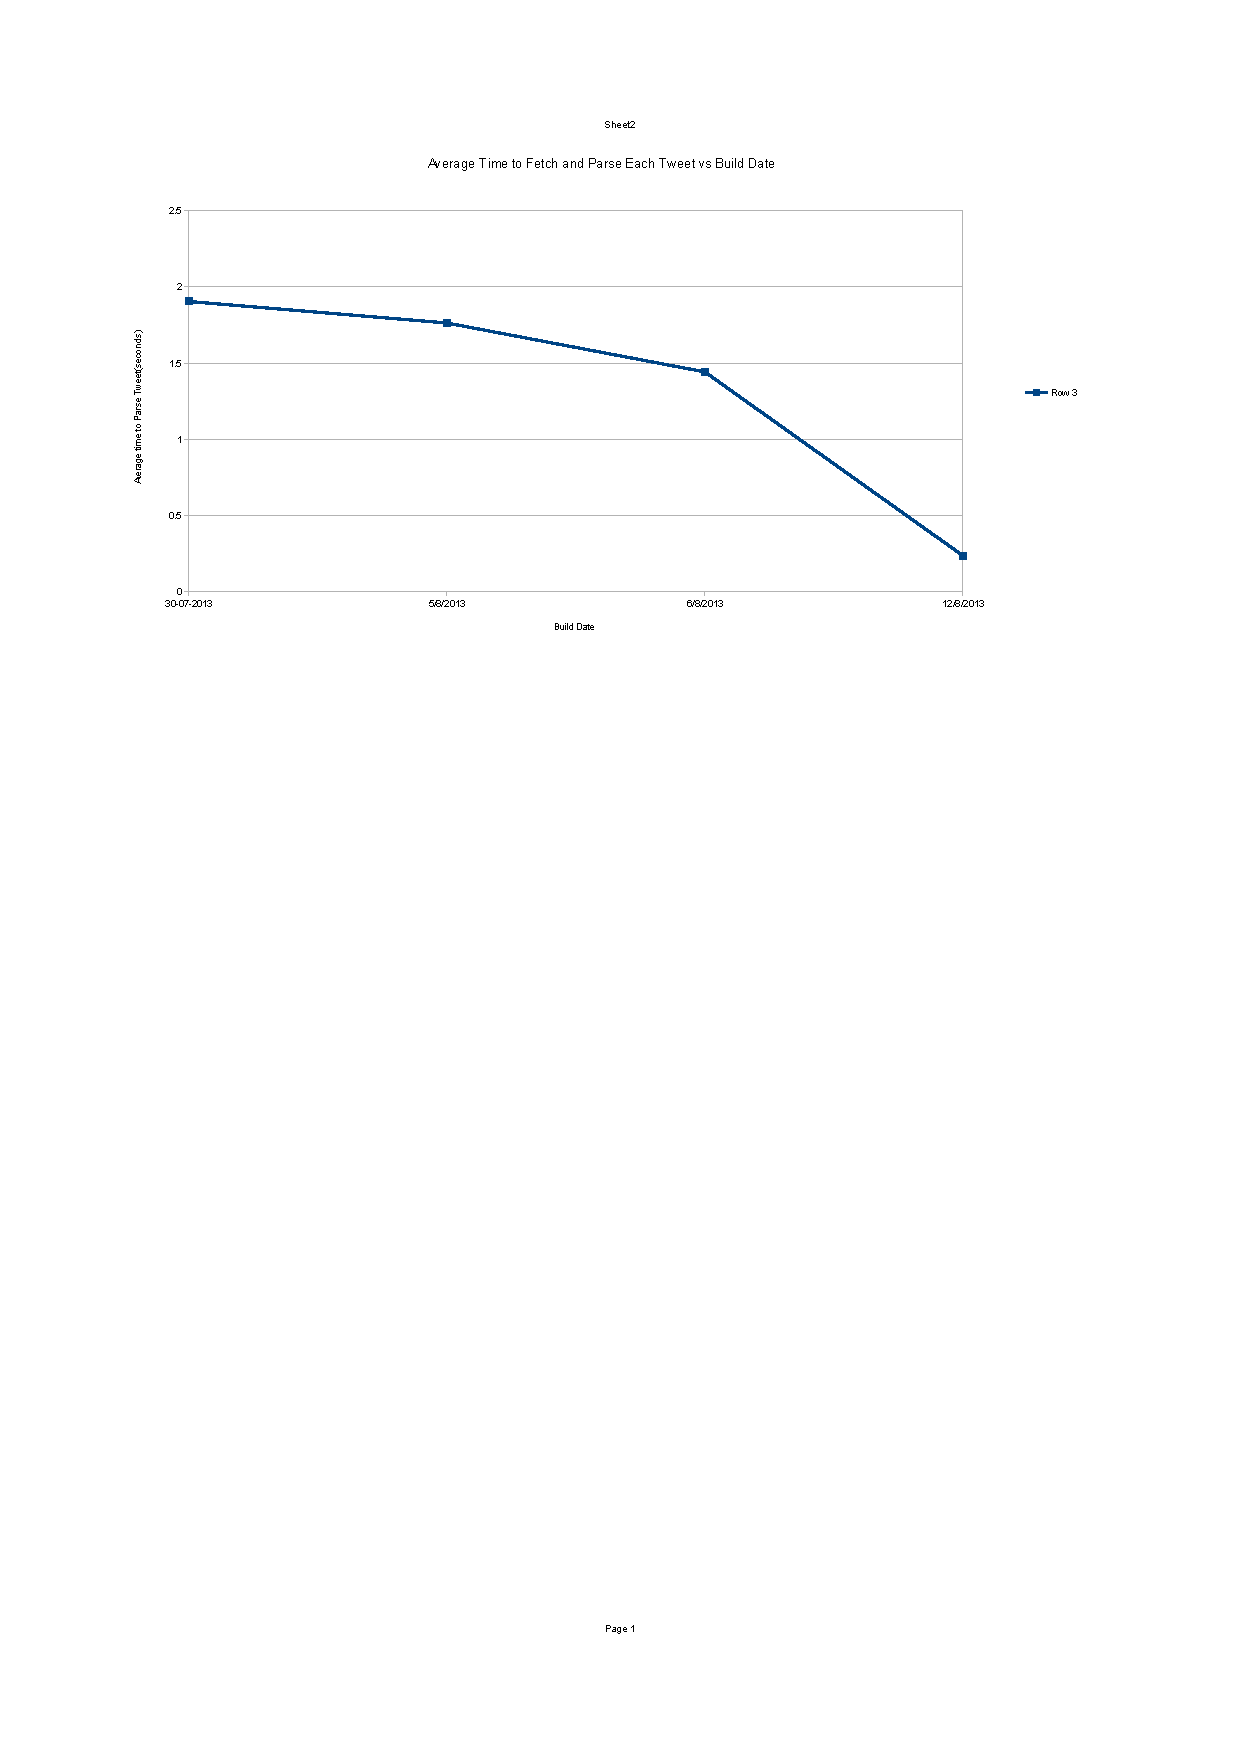
\includegraphics{Images/average_time_to_fetch_parse_tweets_per_build.pdf}
\caption{The Average Time to Fetch and Parse a Tweet, Ordered by Builds}
\end{figure}

Absolute limitations - Every tweet has to be fetched in an individual http request. This produces upper limits as to how fast the scraper can go, and means that the majority of performance speed is reliant on the speed of the network. (data - show how on some days tweets are fetched slightly faster than on other days. Times of day.)

Sensitivity of tweets fetched - it isn't actually much faster if I bulk-collect tweets in a larger 'window', as the majority of time is spent fetching the details of each tweet. 

Parellization of this? Would actually be a useful way of improving speeds...

Discuss why I did not consider parellization at the beginning. The number of requests may be too many and result in more frequent failures than otherwise. Will have to collect the data to verify this claim. 

\subsubsection{Ability to Resist Blocking Detection}

The primary measure of my scraper libraries avoiding blocking detection is with regards to their failure or incomplete-scrape rates. Although in early, less stable builds I had parsing errors, my later work only failed when detected by twitter and blocked. As such detection rates in later builds can reliably be calculated by analysing failing or incomplete twitter profiles. 

\begin{figure}[h!]
\centering
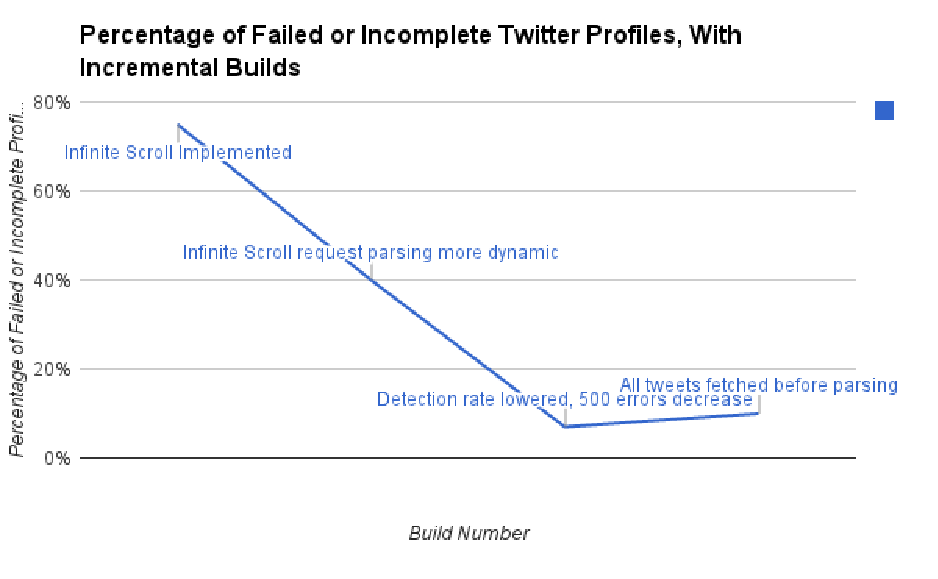
\includegraphics{Images/percentage_failed_incomplete_twitter_profiles.pdf}
\caption{The Percentage of Incomplete or Failed Profile Scrapes, Ordered by Builds}
\end{figure}

\subsubsection{Privacy Protection}

Privacy protection - this is still pretty poor, saved as structured xml, data not anonymised (makes my life easier at present)... Are there things I could be doing here potentially to increase privacy for individuals that I am scraping? Document locking, or store as RDB? Since I plan on storing this info in Graft, this could be anonymised at this point. Individual profiles and what-not. 


